\section{Cruscotto di valutazione della qualità}
\subsection{Qualità di processo}
\subsubsection{MPC01-EAC (Estimated at Completition)}
\begin{figure}[H]
  \centering
  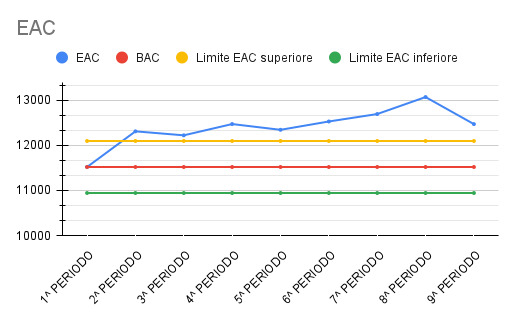
\includegraphics[width=0.7\linewidth]{grafici/EAC.png}
  \caption{Estimated at Completition}
\end{figure}
Dal grafico si può notare che l'EAC supera il valore accettabile di quest'ultimo. La causa di questa situazione si può ricondurre ad una scorretta divisione tra ore produttive e individuali e, inoltre, ai lunghi periodi di tempo impiegati a imparare le $\textit{tecnologie}_G$ necessarie per lo svolgimento del progetto. Si può notare un andamento finale decrescente, quindi si ritiene che dopo la fase iniziale, il gruppo possa rientrare nei valori ottimali. Infine il team è consapevole che l'andamento iniziale del valore è dovuto ad una gestione errata del progetto e quindi i membri dovranno impegnarsi per rientrare nel valore ottimale e garantire il raggiungimento degli obiettivi fissati.

\subsubsection{MPC02-PV (Planned Value) e MPC04-EV (Earned Value)}
\begin{figure}[H]
  \centering
  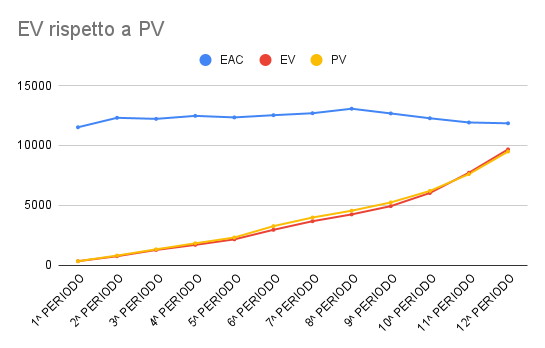
\includegraphics[width=0.7\linewidth]{grafici/EV_PV.png}
  \caption{Planned Value - Earned Value}
\end{figure}
Dal grafico si può notare che le linee del PV e dell'EV sono molto vicine anche se si può notare un allontanamento dei due valori negli ultimi periodi. Questo denota che il costo preventivato è maggiore del costo sostenuto dal gruppo e quindi il team dovrà impegnarsi maggiormente per terminare le attività stabilite.
\subsubsection{MPC05-ETC (Estimated to Complete)}
\begin{figure}[H]
  \centering
  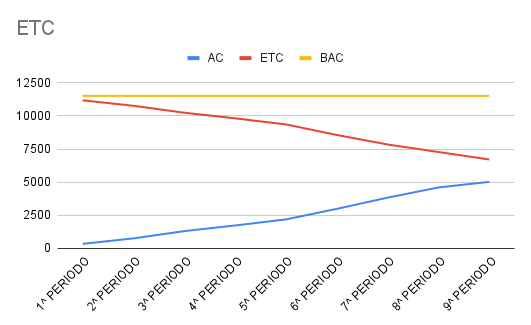
\includegraphics[width=0.7\linewidth]{grafici/ETC.png}
  \caption{Estimated to Complete}
\end{figure}
Dal grafico si può notare che le linee dell'AC e dell'ETC nel corso dei vari periodi, mantengano un andamento costante. Di conseguenza si può affermare che il progetto stia mantenendo un ritmo regolare di avanzamento. 
\subsubsection{MPC06-CV (Cost Variance), MPC07-SV (Schedule Variance) e MPC08-BV (Budget Variance)}
\begin{figure}[H]
  \centering
  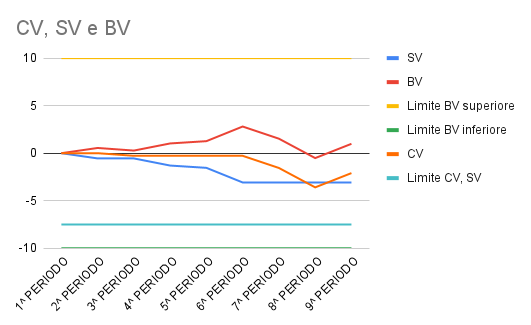
\includegraphics[width=0.7\linewidth]{grafici/CV_SV_BV.png}
  \caption{Cost Variance - Schedule Variance - Budget Variance}
\end{figure}
Dal grafico si può notare che la linea della Cost Variance ha mantenuto un andamento costante e lineare fino al sesto periodo, cosa positiva. Dal settimo periodo periodo però c'è stato un calo, ciò si può ricondurre alla quasi assente divisione delle ore produttive da quelle individuali. Osservando la Schedule Variance si nota invece che l'allontanamento dal valore preferibile è iniziato molto prima. Questa situazione è stata causata da un misto di mancata divisione delle ore produttive e ore individuali, e di sottostime delle ore da dare per ogni lavoro. Infine, osservando la Budget Variance, si nota che, nonostante si sia speso più di quanto previsto per la maggior parte del tempo, ciò si è stabilizzato negli ultimi periodi.
%\subsection{MPC09-RSI (Requirements stability index)}
%\subsection{MPC14-IG (Indice Gulpeanse)}
\subsubsection{MPC09-RSI (Requirements stability index)}
% TO DO
\subsubsection{MPC15-PCTS (Percentuale dei test superati)}
% TO DO
\subsubsection{MPC16-SC (Statement coverage)}
% TO DO
\subsubsection{MPC17-BC (Branch coverage)}
% TO DO
\subsubsection{MPC19-NCR (Non Calculated Risk)}
\begin{figure}[H]
  \centering
  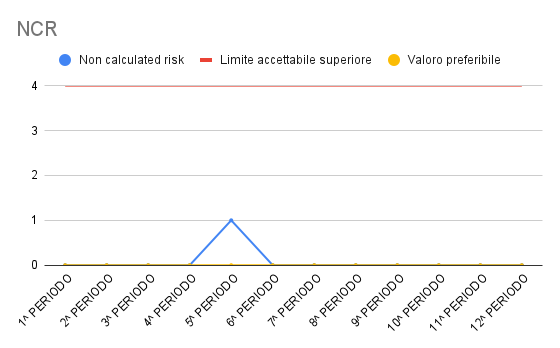
\includegraphics[width=0.7\linewidth]{grafici/NCR.png}
  \caption{Non Calculated Risk}
\end{figure}
Dal grafico si può notare che per la maggior parte del tempo non sono comparsi $\textit{rischi}_G$ non previsti. Solo nel quinto periodo è emerso un $\textit{rischi}_G$o di cui non si era tenuto conto inizialmente, ovvero la sessione di esami, la quale ha portato via parecchio tempo ai vari membri del gruppo, rallentando di molto l'avanzamento del lavoro.
%\subsection{MPC16-ET (Efficienza temporale)}
\subsection{Qualità di prodotto}
\subsubsection{MPD01-CRO (Copertura dei requisiti obbligatori)}
% TO DO
\subsubsection{MPD02-CRD (Copertura dei requisiti desiderabili)}
% TO DO
\subsubsection{MPC07-FD (Failure Density)}
% TO DO